\documentclass[unicode,11pt,a4paper,oneside,numbers=endperiod,openany]{scrartcl}

\usepackage{ifthen}
\usepackage[utf8]{inputenc}
\usepackage{graphics}
\usepackage{graphicx}
\usepackage{hyperref}
\usepackage{amsmath}

\pagestyle{plain}
\voffset -5mm
\oddsidemargin  0mm
\evensidemargin -11mm
\marginparwidth 2cm
\marginparsep 0pt
\topmargin 0mm
\headheight 0pt
\headsep 0pt
\topskip 0pt        
\textheight 255mm
\textwidth 165mm

\newcommand{\duedate} {}
\newcommand{\setduedate}[1]{%
\renewcommand\duedate {Due date:~ #1}}
\newcommand\isassignment {false}
\newcommand{\setassignment}{\renewcommand\isassignment {true}}
\newcommand{\ifassignment}[1]{\ifthenelse{\boolean{\isassignment}}{#1}{}}
\newcommand{\ifnotassignment}[1]{\ifthenelse{\boolean{\isassignment}}{}{#1}}

\newcommand{\assignmentpolicy}{
\begin{table}[h]
\begin{center}
\scalebox{0.8} {%
\begin{tabular}{|p{0.02cm}p{16cm}|}
\hline
&\\
\multicolumn{2}{|c|}{\Large\textbf{Numerical Computing 2022 ---  Submission Instructions}}\\
\multicolumn{2}{|c|}{\large\textbf{(Please, notice that following instructions are mandatory: }}\\
\multicolumn{2}{|c|}{\large\textbf{submissions that don't comply with, won't be considered)}}\\
&\\
\textbullet & Assignments must be submitted to \href{https://www.icorsi.ch/course/view.php?id=14666}{iCorsi} (i.e. in electronic format).\\
\textbullet & Provide both executable package and sources (e.g. C/C++ files, Julia). 
If you are using libraries, please add them in the file. Sources must be organized in directories called:\\
\multicolumn{2}{|c|}{\textit{Project\_number\_lastname\_firstname}}\\
& and  the  file must be called:\\
\multicolumn{2}{|c|}{\textit{project\_number\_lastname\_firstname.zip}}\\
\multicolumn{2}{|c|}{\textit{project\_number\_lastname\_firstname.pdf}}\\
\textbullet &  The TAs will grade your project by reviewing your project write-up, and looking at the implementation you attempted, and benchmarking your code's performance.\\

\textbullet & You are allowed to discuss all questions with anyone you like; however: (i) your submission must list anyone you discussed problems with and (ii) you must write up your submission independently.\\
\hline
\end{tabular}
}
\end{center}
\end{table}
}
\newcommand{\punkte}[1]{\hspace{1ex}\emph{\mdseries\hfill(#1~\ifcase#1{Points}\or{Points}\else{Points}\fi)}}


\newcommand\serieheader[6]{
\thispagestyle{empty}%
\begin{flushleft}

\includegraphics[width=0.45\textwidth]{CI_logo}
\end{flushleft}
  \noindent%
  {\large\ignorespaces{\textbf{#1}}\hspace{\fill}\ignorespaces{ \textbf{#2}}}\\ \\%
  {\large\ignorespaces #3 \hspace{\fill}\ignorespaces #4}\\
  \noindent%
  \bigskip
  \hrule\par\bigskip\noindent%
  \bigskip {\ignorespaces {\Large{\textbf{#5}}}
  \hspace{\fill}\ignorespaces \large \ifthenelse{\boolean{\isassignment}}{\duedate}{#6}}
  \hrule\par\bigskip\noindent%  \linebreak
 }

\makeatletter
\def\enumerateMod{\ifnum \@enumdepth >3 \@toodeep\else
      \advance\@enumdepth \@ne
      \edef\@enumctr{enum\romannumeral\the\@enumdepth}\list
      {\csname label\@enumctr\endcsname}{\usecounter
        {\@enumctr}%%%? the following differs from "enumerate"
	\topsep0pt%
	\partopsep0pt%
	\itemsep0pt%
	\def\makelabel##1{\hss\llap{##1}}}\fi}
\let\endenumerateMod =\endlist
\makeatother




\usepackage{textcomp}

% Math
\usepackage[fleqn]{amsmath}
\usepackage{amssymb}
\usepackage{dsfont}
\usepackage{float}


% Allows to use caption*
\usepackage{caption}
% Scalabale subfigures
\usepackage{subcaption} 
% Code syntax highlighting
\usepackage{minted}
% Hyperlinks
\usepackage{hyperref}


\newcommand{\bmat}[1]{
   \ensuremath{
   \begin{bmatrix}
       #1
   \end{bmatrix}
}}



\usepackage{xcolor}


\begin{document}


\setassignment
\setduedate{Wednesday, 7 December 2022, 11:59 PM}

\serieheader{Numerical Computing}{2022}{Student: Albert Cerfeda}{}{Solution for Project 5}{}
\newline

\assignmentpolicy


The purpose of this assignment is to gain insight on the theoretical and numerical properties of the \textbf{Conjugate Gradient method}. Here we use this method in an image processing application with the goal of \textbf{deblurring} an image given the exact (\textit{noise-free}) blurred image and the original transformation matrix. Note that the ``noise-free" simplification is essential for us to solve this problem in the scope of this assignment.
\tableofcontents
\clearpage


\section{General Questions [10 points]}
\subsection*{1.1. Size of matrix $A$}
$A$ is the sparse symmetric transformation matrix computed by repeateadly applying the \textit{image kernel matrix}\footnote{Image Kernel Matrix: It is a small matrix 
used to transform and apply effects (eg "\textit{filters}") to images. It can be therefore used for applying sharpening,desharpening,embossing ecc. It calculates the new value of a pixel through a weighted sum of the pixel and its neighbors.)}.\\
$B \in \mathds{R}^{n\times n}$ in our case is the transformed,blurred image of size $n$ by $n$ pixels obtained by transforming the original deblurred image $X$ by the transformation matrix $A$.\\
The blurring computation can therefore be defined with the following linear equation:
$$
Ax = b
\label{Eq:system}
$$\\
where $x,b\in \mathds{R}^{n^2}$ are the vectorized representations of original image $X$ and blurred image $B$ respectively, given that $A$ is a square matrix of size $n^2\times n^2$ where $n$ is the size of the image along any dimension.\\
The Julia code for retrieving the size of matrix $A$ is rather trivial:\\
\begin{figure}[H]
\begin{minted}[frame=lines,framesep=2mm,]{julia}
# Load default image data
B = read(matopen("./Data/Blur/B.mat"), "B");
img = B;
n = size(img, 1)
sizeA = n*n
\end{minted}

\caption{Julia code for computing the size of transformation matrix $A$ given blurred image $B$}
\end{figure}
Matrix $A$ is a $62500 \times 62500$ matrix.

\subsection*{1.2. Diagonal bands of matrix $A$}
We know that $A$ is a \textit{$d^2$-banded}\footnote{Banded Matrix: A band matrix is a sparse matrix whose non-zero entries are stored on the main diagonal and zero or more diagonals on each side.} \textbf{symmetric} square matrix where $d$ is the size of the kernel image matrix $K\in \mathds{R}^{d\times d}$. This makes it easy to compute the amount of bands:\\
Since we know that our kernel image matrix is of size $7 \times 7$, our transformation matrix $A$ has $d^2$ bands i.e $49$ bands.




\subsection*{1.3. Lenght of vectorized blurred image $b$}
We require the blurred image $B\in\mathds{R}^{n\times n}$ to be converted into a \textit{vectorized} column vector $b\in\mathds{R}^{n^2}$ for transforming it with transformation matrix $A$.\\
We know that $n = 256$, therefore $n^2=62500$.

\clearpage
\section{Properties of A [10 points]}
\subsection*{2.1 Effects on $\tilde{A}$ when $A$ is not symmetric}
Since $A$ is not positive-definite, we require the computation of $\tilde{A}$ for using the \textit{Conjugate Gradient} method when solving the before-mentioned linear system [Eq. \ref{Eq:system}].\\\\
The \textit{augmented system} is defined as follows:\\
\begin{figure}[h!]
    \centering
    $$
        \underbrace{A^TA}_{\tilde{A}}x = \underbrace{A^Tb}_{\tilde{b}}
    $$
\caption{The \textit{augmented system}}
\label{fig:augmented_system}
\end{figure}\\
We compute the augmented system when the coefficient matrix $A$ is not positive definite, like in our case.
This operation affects the \textit{condition number} $\kappa(A)$ [See Section \hyperref[condition_number]{3.3}] as $\kappa(\tilde{A}) \approx \kappa(A)^2$. 

Was matrix $A$ not to be symmetric, its augmented counterpart would still be symmetric as any square matrix $B$ multiplied by its transposed $B^T$ i.e $B^TB$ is symmetric. 

% TODO: [X] 2.1 Effects when A is not symmetric


\subsection*{2.2 Proof for the minimization problem}
We need to show that the solving $Ax=b$ is equal to minimizing $\frac{1}{2}A^Tx+\frac{1}{2}Ax-b$ over $x$.\\
Let us compute the derivative $f'(x) = \frac{d}{dx}\frac{1}{2}A^Tx+\frac{1}{2}Ax-b$.\\
\begin{align*}
    f'(x)&= \frac{1}{2}A^Tx+\frac{1}{2}Ax-b\\
    &= \frac{1}{2}Ax+\frac{1}{2}Ax-b\\
    &= Ax-b \\
\end{align*}
\textbf{Note:} Since matrix $A$ is symmetric, $A^T=A$.\\
We can see how computing the derivative and then substituting $A^T$ with $A$ leads to equation $Ax=b$, therefore proving the above statement.


% TODO: 2.2 Proof Answer


\section{Conjugate Gradient [30 points]}
\subsection*{3.1 Conjugate Gradient solver implementation}
We want to find the original,deblurred image $X$ by solving the linear system that represents the blurring operation [See Eq. \ref{Eq:system}] by the vectorized image $x$, given that transformation matrix $A$ and vectorized blurred image $b$ are known.\\

The methods for computing a linear system fall under two main categories: \textit{Direct methods} and \textit{Iterative methods}.\\
Direct methods find the exact solution (e.g Gaussian Elimination). Gaussian Elimination becomes unfeasably expensive for very large matrices like in our case. Iterative methods on the other hand start with a random solution converging more towards the exact result with each iteration, deriving an approximated result.\\\\

The \textit{Conjugate Gradient solver} is an iterative method for finding an \textit{approximated} solution to a very large linear system of equations like in our case. It's more specific than the Gaussian method as it requires matrix $A$ to be a symmetric, positive-definite matrix.\\

Figure \ref{fig:myCG} shows the implementation of \verb|function myCG(A,b,x0,max_itr,abstol)|:\\\\
\textbf{Note:} Input parameter \verb|tol| was renamed to \verb|abstol| to avoid confusion.\\
Function \verb|IterativeSolvers.cg(A, b; kwargs...)|\footnote{IterativeSolvers.cg(...): See documentation 
\href{https://iterativesolvers.julialinearalgebra.org/stable/linear_systems/cg/\#CG}{iterativesolvers.julialinearalgebra.org} 
} features named parameters \verb|abstol| and \verb|reltol| for specifying either the relative tolerance ratio between iterations or the absolute tolerance value. Since in our implementation we are effectively using the absolute tolerance for probing convergence, the parameter was renamed to ensure consistency.\\

\begin{figure}[h!]
    \begin{minted}[frame=lines,framesep=2mm,]{julia}
function myCG(A,b,x0,max_itr,abstol)
    rvec = [];
    x = x0;
    r = b-A*x;
    d = r;
    p_old = dot(r,r)
    for i in 1:max_itr
        s = A*d;
        alpha = p_old / dot(d,s);
        x = x + alpha*d;
        r = r - alpha*s;
        p_new = dot(r,r);
        beta = p_new / p_old;
        d = r + beta*d;
        p_old = p_new;
        
        push!(rvec,p_new);
        if sqrt(p_new) <= abstol
            println("Converged")
            break
        end
    end
    return x, rvec
end
\end{minted}

    \caption{Julia code defining the implementation of the \textit{Conjugate Gradient solver} }
    \label{fig:myCG}
\end{figure}

\subsection*{3.2 Solving the system defined by  \textit{A\_test.mat} and \textit{b\_test.mat}}
Let us solve the provided sample linear system: %[Figure \ref{fig:solveLinearEq}]
\begin{figure}[H]
    \begin{subfigure}[l]{\textwidth}
\begin{minted}[frame=lines,framesep=2mm,]{julia}

# Load test data
b_test = read(matopen("./Data/Test/b_test.mat"), "b_test");
img = b_test

# Blurred image
heatmap(reshape(img, (10, 10)), c=:greys, yflip=true,
    legend=:none, axis=nothing, aspect_ratio=:equal, xlabel="Blurred")

# Load transformation matrix A
A_test = read(matopen("./Data/Test/A_test.mat"), "A_test");

## Run myCG() on B_test
guess = ones(size(A_test,1));
maxiter = 200;
abstol = 1e-4;

x,residuals = myCG(A_test,b_test,guess,maxiter,abstol)
# Deblurred image
heatmap(reshape(x, (10, 10)), c=:greys, yflip=true, 
    legend=:none, axis=nothing, aspect_ratio=:equal, xlabel="Deblurred")

## Plot convergence
plot(residuals,  ylims=(-Inf,1e5), xlabel="Iterations",ylabel="Residual value",
    yscale=:log10)
\end{minted}
    \end{subfigure}
    \caption{Julia code solving the sample linear system by using function \textit{myCG} [Fig. \ref{fig:myCG}]}
    \label{fig:solveLinearEq}
\end{figure}

Let us plot the blurred and the obtained deblurred counterpart:
\begin{figure}[!h]
    \begin{minipage}{0.5\textwidth}
        \centering
        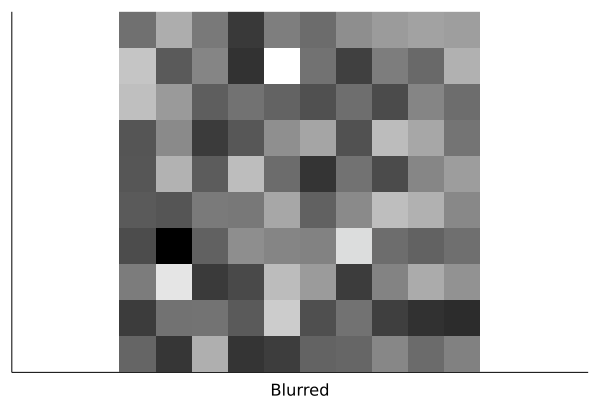
\includegraphics[width=0.6\linewidth]{fig/out/3.2-'B-test'-blurred.png}
    \end{minipage}
        \begin{minipage}{0.5\textwidth}
        \centering
        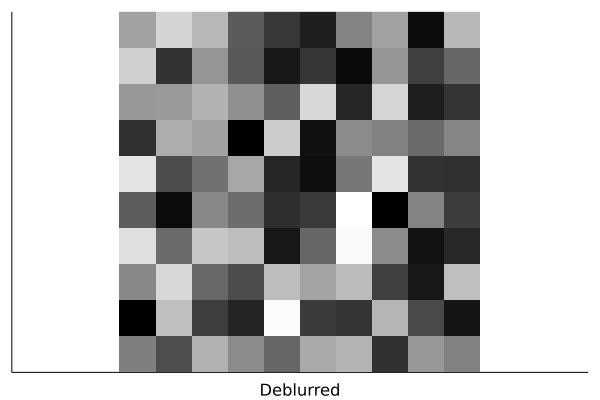
\includegraphics[width=0.6\linewidth]{fig/out/3.2-'B-test'-deblurred.png}
    \end{minipage}
    \caption{The \textit{B\_test} image. On the left, the blurred one. On the right, the deblurred image obtained though function \textit{myCG} [Fig. \ref{fig:myCG}]}
\end{figure}\\
Its difficult to verify the correctness solely from the visual comparison as the images are too low-resolution for us to intuitively detect correct deblurring. However, convergence is achieved as shown by the plot representing the residual value variation [See Fig.\ref{fig:residual_variation}]:

\begin{figure}[h!]
    \centering
    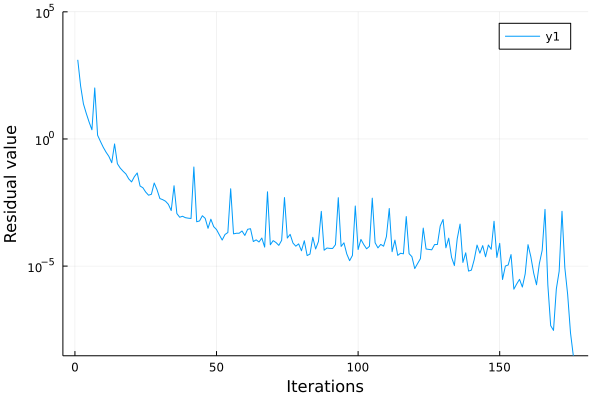
\includegraphics[width=0.8\linewidth]{fig/out/3.2-'B-test'-convergence.png}
    \caption{Plot representing the residual value variation for each iteration}
    \label{fig:residual_variation}
\end{figure}
It can be observed how the \textit{Conjugate Gradient solver} method quickly finds convergence in few iterations.

\subsection*{\normalsize{3.3 Condition number and convergence rate in relation to the Eigenvalues of \textit{A\_test.mat}}}
\label{condition_number}
The condition number $\kappa (A)$ is a property on linear systems of equations. It measures how much the result of the equation changes in respect to the input arguments. A system with a high condition number is called \textit{"ill-conditioned"}, implying that it is harder to compute a solution. A system with a low condition number is instead called \textit{well-conditioned}.\\
The condition number directly affects the convergence rate of the \textit{Conjugate Gradient} method, as running it on an ill-contitioned system results in significantly lower convergence rate.\\
The \textit{Condition Number} of a square matrix is defined as follows:\\
$$
\kappa (A) = \frac{\sigma_{\text{max}}}{\sigma_{\text{min}}} \qquad \text{where $\sigma$ are the singular values of matrix $A$}
$$
The singular values of a symmetric matrix are equal to the absolute values of its eigenvalues, i.e $\sigma = |\lambda|$. This property holds for our transformation matrix $A$ as it is symmetrical.\\
We can intuitively infer from the previous statements that the condition number of a system comes from the maximal ratio between eigenvalues of the \textit{coefficient matrix} of the system (e.g matrix $A$ [See Eq.\ref{Eq:system}])\\
Let us plot the eigenvalues of provided transformation matrix \verb|A_test.mat|
\begin{figure}[H]
    \centering
    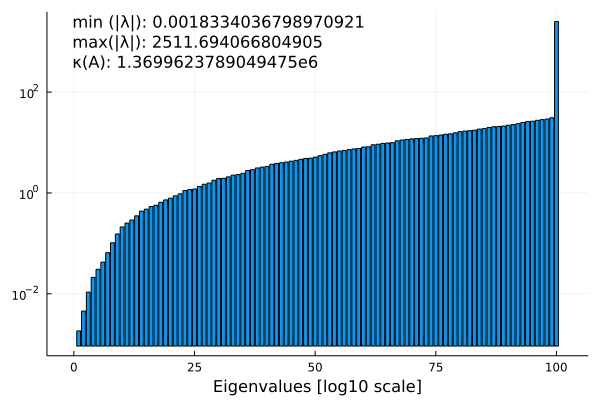
\includegraphics[width=0.7\linewidth]{fig/out/3.2-'B-test'-eigvals.png}
    \caption{Bar graph representing the residual value variation for each iteration when running function \textit{myCG} on matrix \textit{A\_test.mat} and vectorized blurred image \textit{b\_test.mat}, in \textit{log10} scale}
    \label{fig:eigvals}
\end{figure}
As we can see the distance between the smallest absolute eigenvalue $\kappa_{\text{min}}$ and the greatest absolute eigenvalue $\kappa_{\text{max}}$ is rather large. In fact $\kappa (A) \approx 1.37*10^6$.\\
The condition number gets drastically worse if matrix \verb|A_test.mat|  was not to be positive definite, requiring us to solve for the \textit{augmented system} $\tilde{A}x =  \tilde{b}$ where $\tilde{A} = A^TA$ and $\tilde{b} = A^Tb$, making the condition number grow exponentially. This case does not present itself as matrix \verb|A_test.mat| is already positive definite.\\
We can use a technique known as \textit{preconditioning} for reducing the distance of the eigenvalues and therefore lower the condition number.\\
\subsection*{3.4 Residual variation non-monotonically decreasing}
As we can see from Figure \ref{fig:eigvals}, the residual variation is \textit{not} decreasing monotonically. \\
Function \verb|myCG| minimizes the distance of the vectorized unblurred image $x$ from the actual vectorized unblurred image (the optimal $x$). This makes the residual variation generally decrease like expected leading towards convergence, but not monotonically.\\
Instead, if function \verb|myCG| was to minimize the residual, the residual variation would decrease monotonically.\\

\section{Deblurring problem [35 points]}
\subsection*{4.1 Preconditioning using the \textit{incomplete Cholesky factorization}}
As mentioned before the condition number directly depends on the \textit{range} of the eigenvalues of the coefficient matrix (eg transformation matrix $A$), given that it is a symmetric matrix.\\
An already adverse condition number $\kappa (A)$ only gets worse if we take in account some pre-manipulation done on system, like computing the \textit{augmented system} [See Fig \ref{fig:augmented_system}].\\\\

The \textit{Identity Matrix} $I\in \mathds{R}^{n\times n}$ by definition has $n$ eigenvalues valued $1$ (i.e $\lambda_{1,..n} = 1$). This ensures the lowest possible distance between eigenvalues and therefore $\kappa(A) = \frac{1}{1} = 1$. The condition number being equal to $1$ implies that the algorithm will not arbitrarily diverge because of errors in the input and that the precision of the approximated result will be no different from the precision of the input data.\\
\label{preconditioning_par}
We can find matrix $P^{-1}$ that approximates $\tilde{A}^{-1}$ meaning that once multiplied, the resulting matrix is closer to the Identity Matrix i.e:
$$
P^{-1}\tilde{A} \approx I \quad \text{where $P$ is the symmetric positive-definite \textit{preconditioner}}
$$ 
By approximating $\tilde{A}$ to the identity matrix $I$ we ensure a smaller eigenvalue range and a lower condition number $\kappa(A)$. This technique is known as \textit{preconditioning}.\\
We can decompose the preconditioner $P$ such that $P= LL^T$, where $L$ is the Cholesky Factor.\\

The Cholesky factorization decomposes a matrix $A$ into a lower-triangular matrix $L$ and its upper-triangular counterpart $L^T$. For sparse matrices, we use the \textit{Incomplete} Cholesky factorization, a sparse approximation of the regular method. It computes the Cholesky factors of only the non-zero elements of $A$ resulting in cheaper computational cost for sparse matrices.\\


Finally we can implement the Julia script for deblurring the provided \verb|B.mat| image. The transformation matrix $A$ has to be first augmented to ensure symmetricity and then shifted by $0.01$ along its diagonal to ensure the existance of IC factors. After that, the final steps are rather trivial: we make use of the \verb|CholeskyPreconditioner(..)| function inside package \verb|Preconditioners.jl|\footnote{Preconditioners.CholeskyPreconditioner(..): See codebase [\href{https://github.com/JuliaLinearAlgebra/Preconditioners.jl}{github.com}]}\\
As requested the \textit{maximum iterations} is set to $200$ and the \textit{absolute tolerance} to $10^{-4}$. The Julia code is shown in Figure \ref{B_mat_deblur_JULIA}.\\

\begin{figure}[H]
\begin{minted}[frame=lines,framesep=2mm,]{julia}
# Load blurred image B
B = read(matopen("./Data/Blur/B.mat"), "B");
img = B;
n = size(img, 1)
# Vectorize image
b = vec(B)
# Load transformation matrix A
A = read(matopen("./Data/Blur/A.mat"), "A");

# The initial guess
guess = ones(size(b,1));
# The maximum amount of iterations
maxiter = 200;
# The absolute tolerance
abstol = 1e-4;

# Compute augmented matrix to ensure positive-definedness and symmetricity
augA = A'A
# Shift diagonal by 0.01 to ensure the existance of IC factors
augA = 0.01*I+augA
# Retrieve the Cholesky preconditioner matrix with memory fill set to 1
P = CholeskyPreconditioner(augA,1);

# Run function IterativeSolvers.cg(...)
x, residuals  = IterativeSolvers.cg(A,b,log=true,Pl=P,maxiter=maxiter,abstol=abstol)
# Run function myCG()
x,residuals = myCG(A,b,guess,maxiter,abstol)
\end{minted}
        \caption{Julia code for deblurring the provided blurred $\texttt{B.mat}$ image with both function $\texttt{myCG()}$ [Fig.\ref{fig:myCG}] and $\texttt{IterativeSolvers.cg(...)}$}
        \label{B_mat_deblur_JULIA}
\end{figure}


Let us plot the obtained deblurred images with the respective methods: [See \hyperref[fig:B_mat_deblur]{results}]

\begin{figure}[h!]
    \centering
    \begin{minipage}{.8\textwidth}
        \centering
        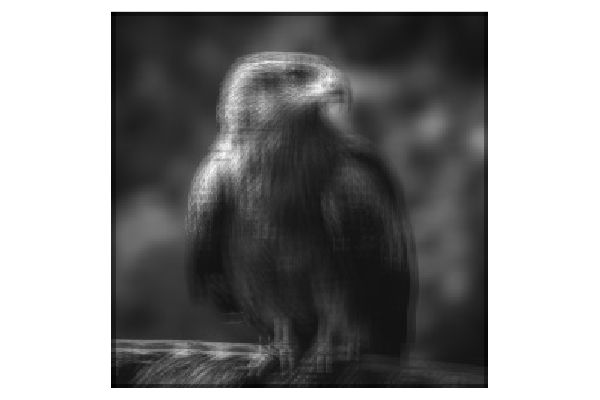
\includegraphics[width=0.9\linewidth]{fig/out/4.1-'B'-blurred.png}
        \caption{Provided blurred image $\texttt {B.mat}$}    
    \end{minipage}

    \begin{minipage}{.8\textwidth}
        \centering
        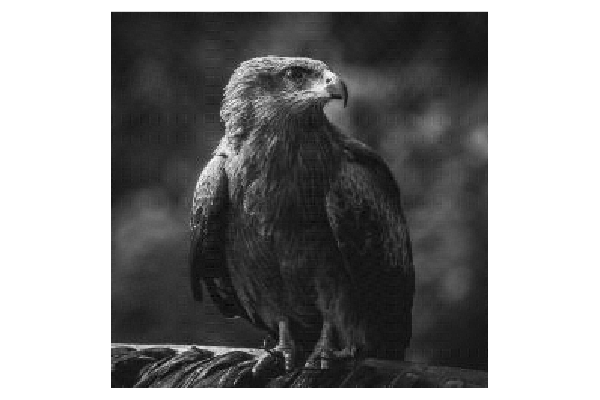
\includegraphics[width=.9\linewidth]{fig/out/4.1-'B'-'cg()'-deblurred.png}
        \caption{\small Obtained deblurred image using function $\texttt {IterativeSolvers.cg(...)}$}
    \end{minipage}
    \begin{minipage}{.8\textwidth}
        \centering
        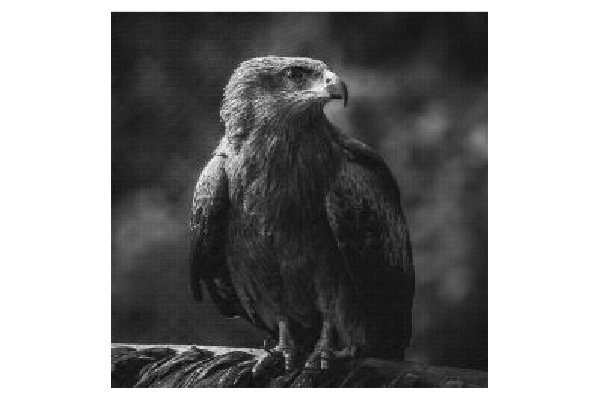
\includegraphics[width=.9\linewidth]{fig/out/4.1-'B'-'myCG()'-deblurred.png}
        \caption{Obtained deblurred image using function $\texttt {myCG(...)}$}
    \end{minipage}
    \label{fig:B_mat_deblur}
    % \caption*{}
\end{figure}
We can clearly see how the implementation is correct as the images are correctly deblurred. Both methods do not converge, as 200 iterations in this instance are too few. Nevertheless, we still obtain a sufficiently deblurred image.\\

Plotting the residual value variation yields the following results [See \hyperref[fig:B_mat_convergence]{results}].\\
Even tough both methods do not converge we notice how the residual variation is way lower in Figure \ref{fig:B_mat_convergence_CG}. This is clearly due to the benefits of performing preconditioning on the augmented matrix $\tilde{A}$. As stated before\ref{preconditioning_par} the preconditioning step is performed to approximate $\tilde{A}$ to the identity matrix $I$ to ensure a smaller eigenvalue range and a lower condition number $\kappa(A)$.



\begin{figure}[h!]
    \begin{minipage}{.5\textwidth}
        \centering
        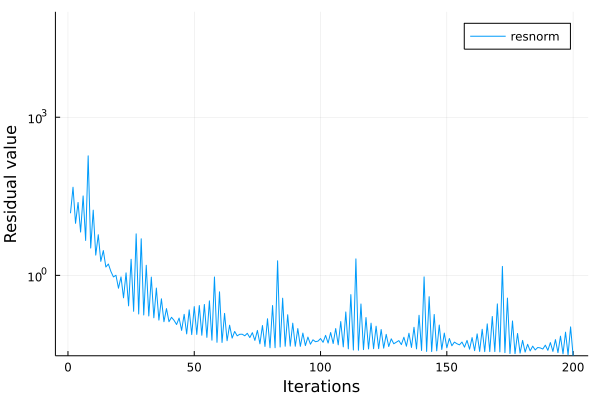
\includegraphics[width=1.1\linewidth]{fig/out/4.1-'B'-'cg()'-convergence.png}
        \caption{\small Obtained deblurred image using function $\texttt {IterativeSolvers.cg(...)}$}
        \label{fig:B_mat_convergence_CG}
    \end{minipage}
    \begin{minipage}{.5\textwidth}
        \centering
        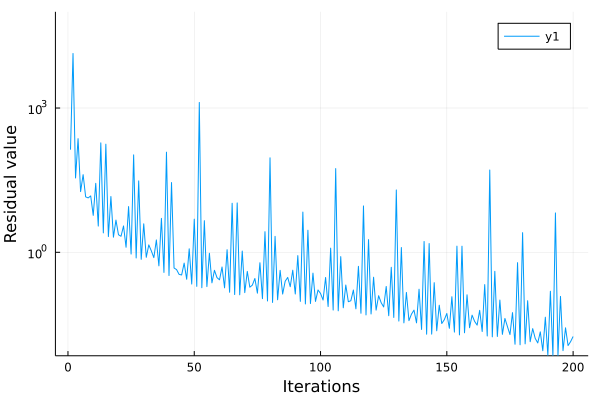
\includegraphics[width=1.1\linewidth]{fig/out/4.1-'B'-'myCG()'-convergence.png}
        \caption{Obtained deblurred image using function $\texttt {myCG(...)}$}
    \end{minipage}
    \label{fig:B_mat_convergence}
    % \caption*{}
\end{figure}

% TODO: 4.1 Answer

\subsection*{4.2 Amortized cost of preconditioned Conjugate Gradient method}
Even though performing the preconditioning step leads to some performance overhead, the overall \textit{amortized} cost in the long run, in the case where the same transformation matrix $A$ is used to deblur multiple images which share a common image kernel matrix, makes it worth using preconditioning given its faster convergence rate.
% TODO: 4.2 Answer

\section{Reproducing the obtained results}
In the \verb|src/| folder inside the submission archive you can find a \verb|Makefile|.\\\\
Run command \verb|make| while having the current working directory set as the \verb|src/| folder to plot and store all the results used for this report. All the plots and blurred/unblurred images are saved inside the \verb|src/out| folder. Make sure to uncomment the \verb|png(...)| statements for the files you want to generate.\\\\


\end{document}
